%File: anonymous-submission-latex-2024.tex
\documentclass[letterpaper]{article} % DO NOT CHANGE THIS
\usepackage[submission]{aaai24}  % DO NOT CHANGE THIS
\usepackage{times}  % DO NOT CHANGE THIS
\usepackage{helvet}  % DO NOT CHANGE THIS
\usepackage{courier}  % DO NOT CHANGE THIS
\usepackage[hyphens]{url}  % DO NOT CHANGE THIS
\usepackage{graphicx} % DO NOT CHANGE THIS
\urlstyle{rm} % DO NOT CHANGE THIS
\def\UrlFont{\rm}  % DO NOT CHANGE THIS
\usepackage{natbib}  % DO NOT CHANGE THIS AND DO NOT ADD ANY OPTIONS TO IT
\usepackage{caption} % DO NOT CHANGE THIS AND DO NOT ADD ANY OPTIONS TO IT
\frenchspacing  % DO NOT CHANGE THIS
\setlength{\pdfpagewidth}{8.5in} % DO NOT CHANGE THIS
\setlength{\pdfpageheight}{11in} % DO NOT CHANGE THIS
%
% These are recommended to typeset algorithms but not required. See the subsubsection on algorithms. Remove them if you don't have algorithms in your paper.
\usepackage{algorithm}
\usepackage{algorithmic}

%
% These are are recommended to typeset listings but not required. See the subsubsection on listing. Remove this block if you don't have listings in your paper.
\usepackage{newfloat}
\usepackage{listings}
\DeclareCaptionStyle{ruled}{labelfont=normalfont,labelsep=colon,strut=off} % DO NOT CHANGE THIS
\lstset{%
	basicstyle={\footnotesize\ttfamily},% footnotesize acceptable for monospace
	numbers=left,numberstyle=\footnotesize,xleftmargin=2em,% show line numbers, remove this entire line if you don't want the numbers.
	aboveskip=0pt,belowskip=0pt,%
	showstringspaces=false,tabsize=2,breaklines=true}
\floatstyle{ruled}
\newfloat{listing}{tb}{lst}{}
\floatname{listing}{Listing}
%
% Keep the \pdfinfo as shown here. There's no need
% for you to add the /Title and /Author tags.
\pdfinfo{
/TemplateVersion (2024.1)
}

% DISALLOWED PACKAGES
% \usepackage{authblk} -- This package is specifically forbidden
% \usepackage{balance} -- This package is specifically forbidden
% \usepackage{color (if used in text)
% \usepackage{CJK} -- This package is specifically forbidden
% \usepackage{float} -- This package is specifically forbidden
% \usepackage{flushend} -- This package is specifically forbidden
% \usepackage{fontenc} -- This package is specifically forbidden
% \usepackage{fullpage} -- This package is specifically forbidden
% \usepackage{geometry} -- This package is specifically forbidden
% \usepackage{grffile} -- This package is specifically forbidden
% \usepackage{hyperref} -- This package is specifically forbidden
% \usepackage{navigator} -- This package is specifically forbidden
% (or any other package that embeds links such as navigator or hyperref)
% \indentfirst} -- This package is specifically forbidden
% \layout} -- This package is specifically forbidden
% \multicol} -- This package is specifically forbidden
% \nameref} -- This package is specifically forbidden
% \usepackage{savetrees} -- This package is specifically forbidden
% \usepackage{setspace} -- This package is specifically forbidden
% \usepackage{stfloats} -- This package is specifically forbidden
% \usepackage{tabu} -- This package is specifically forbidden
% \usepackage{titlesec} -- This package is specifically forbidden
% \usepackage{tocbibind} -- This package is specifically forbidden
% \usepackage{ulem} -- This package is specifically forbidden
% \usepackage{wrapfig} -- This package is specifically forbidden
% DISALLOWED COMMANDS
% \nocopyright -- Your paper will not be published if you use this command
% \addtolength -- This command may not be used
% \balance -- This command may not be used
% \baselinestretch -- Your paper will not be published if you use this command
% \clearpage -- No page breaks of any kind may be used for the final version of your paper
% \columnsep -- This command may not be used
% \newpage -- No page breaks of any kind may be used for the final version of your paper
% \pagebreak -- No page breaks of any kind may be used for the final version of your paperr
% \pagestyle -- This command may not be used
% \tiny -- This is not an acceptable font size.
% \vspace{- -- No negative value may be used in proximity of a caption, figure, table, section, subsection, subsubsection, or reference
% \vskip{- -- No negative value may be used to alter spacing above or below a caption, figure, table, section, subsection, subsubsection, or reference

\setcounter{secnumdepth}{0} %May be changed to 1 or 2 if section numbers are desired.

\usepackage{amsmath}
\usepackage{amssymb}
\usepackage{amsthm}
\usepackage{todonotes}
\usepackage{bm}
\usepackage{subcaption}
% \usepackage[ruled]{algorithm2e}

\def\ci{\perp\!\!\!\!\!\perp}

\newtheorem{definition}{Definition}
\newtheorem{proposition}{Proposition}
\newtheorem{theorem}{Theorem}


% The file aaai24.sty is the style file for AAAI Press
% proceedings, working notes, and technical reports.
%

% Title

% Your title must be in mixed case, not sentence case.
% That means all verbs (including short verbs like be, is, using,and go),
% nouns, adverbs, adjectives should be capitalized, including both words in hyphenated terms, while
% articles, conjunctions, and prepositions are lower case unless they
% directly follow a colon or long dash
\title{Expert-In-The-Loop Causal Discovery: An Iterative Approach for Efficiently Utilizing Expert Knowledge in Model Modification}
\author{
    %Authors
    % All authors must be in the same font size and format.
    Written by AAAI Press Staff\textsuperscript{\rm 1}\thanks{With help from the AAAI Publications Committee.}\\
    AAAI Style Contributions by Pater Patel Schneider,
    Sunil Issar,\\
    J. Scott Penberthy,
    George Ferguson,
    Hans Guesgen,
    Francisco Cruz\equalcontrib,
    Marc Pujol-Gonzalez\equalcontrib
}
\affiliations{
    %Afiliations
    \textsuperscript{\rm 1}Association for the Advancement of Artificial Intelligence\\
    % If you have multiple authors and multiple affiliations
    % use superscripts in text and roman font to identify them.
    % For example,

    % Sunil Issar\textsuperscript{\rm 2},
    % J. Scott Penberthy\textsuperscript{\rm 3},
    % George Ferguson\textsuperscript{\rm 4},
    % Hans Guesgen\textsuperscript{\rm 5}
    % Note that the comma should be placed after the superscript

    1900 Embarcadero Road, Suite 101\\
    Palo Alto, California 94303-3310 USA\\
    % email address must be in roman text type, not monospace or sans serif
    proceedings-questions@aaai.org
%
% See more examples next
}

%Example, Single Author, ->> remove \iffalse,\fi and place them surrounding AAAI title to use it
\iffalse
\title{My Publication Title --- Single Author}
\author {
    Author Name
}
\affiliations{
    Affiliation\\
    Affiliation Line 2\\
    name@example.com
}
\fi

\iffalse
%Example, Multiple Authors, ->> remove \iffalse,\fi and place them surrounding AAAI title to use it
\title{My Publication Title --- Multiple Authors}
\author {
    % Authors
    First Author Name\textsuperscript{\rm 1},
    Second Author Name\textsuperscript{\rm 2},
    Third Author Name\textsuperscript{\rm 1}
}
\affiliations {
    % Affiliations
    \textsuperscript{\rm 1}Affiliation 1\\
    \textsuperscript{\rm 2}Affiliation 2\\
    firstAuthor@affiliation1.com, secondAuthor@affilation2.com, thirdAuthor@affiliation1.com
}
\fi


\begin{document}

\maketitle

\begin{abstract}
	\emph{Causal Discovery} has received significant attention in the
	Directed Acyclic Graphs (DAGs) literature, leading to the development
	of numerous automated algorithms for constructing DAGs from data.
	Despite these advancements, the application of these algorithms in
	applied domains remain limited, with researchers often preferring to
	construct DAGs manually based on their expert knowledge. We hypothesize
	that the reluctance to use automated algorithms arises due to several
	practical issues, such as difficulty in choosing the best algorithm and
	their hyperparameters for a given dataset, algorithms can make obvious
	mistakes, and they output the Markov Equivalence Class (MEC) instead of
	a DAG, which is often required for further analysis. Even when using
	these algorithms, researchers must rely on their expert knowledge to
	make modifications, or orient edges of the learned model. Given this
	reliance on manual model construction and modification, in this paper,
	we present a method inspired by \emph{specification search} in
	Structural Equation Models (SEMs) to assist researchers in iteratively
	modifying their models. Specifically, we utilize implied Conditional
	Independence (CI) based model testing combined with a novel measure of
	partial association for mixed data to rank violations of implied CIs in
	data. Using this ranking users can make modifications to their models
	by either removing edges or adding edges between pair of variables
	while deciding the direction of the edge based on their domain
	expertise. The ranking allows users to prioritize the worst offending
	violations first. Through empirical analysis, when applied to learning
	the model, we demonstrate that taking a greedy approach (i.e., fixing
	the worst violation first) this approach can get comparable performance
	to automated algorithms if the users are able to get the edge direction
	correctly with an accuracy higher than $ 0.4 $. (check if this is
	correct). Alternatively, we show that a Large Language Model (LLM) can
	also be used to help in deciding the direction between the variables.
\end{abstract}

\section{Introduction}

Understanding the cause-and-effect relationships between variables is a
fundamental goal in many scientific questions as it reveals the underlying
mechanisms of observed phenomena and informs effective interventions or policy
decisions. \emph{Causal Discovery} methods aim to uncover these underlying
cause-effect relationships among random variables from observational data. The
problem of causal discovery has been explored in both the Directed Acyclic
Graphs (DAGs) and Structural Equation Models (SEMs) literatures, each adopting
a different approach. In the DAG literature, the focus has primarily been on
developing automated algorithms that can learn the causal structure from
datasets. As a result of these efforts, numerous algorithms for causal
discovery have been proposed in the DAG literature, such as constraint-based
methods like the PC algorithm \citep{Spirtes2001} and Fast Causal Inference
(FCI) \citep{Spirtes2000}), score-based methods like Hill-Climb Search and
Greedy Equivalence Search (GES) \citep{Chickering2002}, and continuous
optimization-based methods like NO TEARS \citep{Zheng2018} and DAGMA
\citep{Bello2022}. In contrast, the SEM literature has focused more towards
developing tools that can assist researchers in manually constructing or
modifying models by allowing them to integrate their expert knowledge into the
model building process. Researchers typically develop an initial model based on
domain knowledge and use various tools to guide modifications to improve the
fit of their model to data. This model construction process is known as
\emph{Specification Search}. A common method for specification search is using
\emph{modification indices}, which identify potential changes to the model
structure that improve the model fit. These potential changes are then ranked
by the ones that improve the fit the most. This ranking allows the researchers
to focus first on the suggestions that can improve the model the most and while
integrating their expertise to choose the most optimal modifications.

Even though so many automated algorithms have been proposed, the adaption of
these algorithms in applied fields remain limited, and researchers typically
prefer to construct DAGs manually based on their domain expertise
\citep{Tennant2020, Petersen2021}. We believe this is the case because of
problems with these algorithms when applied in practical settings:

\begin{enumerate}
	\item \textbf{Make Obvious Mistakes:} Although most algorithms are
		theoretically consistent asymptotically, their finite sample
		properties are not well understood. Moreover, depending on the
		selected hyperparameters, their output can vary significantly.
		These issues combined with no good method to test the
		performance of these algorithms on a given dataset, in
		real-world settings with finite samples, it can be difficult to
		trust the output of these algorithms. Consequently, researchers
		have to rely on posthoc modifications to the model based on
		their domain expertise.
	\item \textbf{Outputs Markov Equivalence Class (MEC):} Multiple
		DAGs can be faithful to a given observational dataset. Thus,
		using only observational data, algorithms can only recover the
		MECs that can contain a combination of directed and undirected
		edges. However, most methods for downstream tasks, such as
		identification or causal effect estimation, assume knowledge of
		a fully oriented DAG. As a result, researchers have to manually
		orient these edges before using them for analysis.
\end{enumerate}

\todo[inline]{Add an example here showing these problems}

Due to these challenges, even when using automated algorithms, we often have to
rely on manual post hoc testing and modifications to the model learned by the
algorithm. Whether constructing the model manually or using an algorithm, we
must rely on domain expertise to construct or modify the model. Hence, it is
crucial to have tools to guide this modification process. One of the ways to
guide this modification is to use Conditional Independence (CI) based model
testing \cite{Ankan2023}. As DAGs imply CI statements that can be tested in the
given data using statistical CI tests, we can verify whether the implied CIs
are consistent in the data or not. If some of implied CIs are not valid in the
given dataset, we can modify the model accordingly. Figure~\ref{fig:ci_testing}
shows an example of model testing using CIs. However, using p-values of the CI
tests has a few drawbacks. Firstly, as CIs are implied only by missing edges in
the model, we can not test whether an incorrect edge is already present in the
model. For examples, in high sample size scenarios, we might get a significant
association between a pair of variables with very small association. Secondly,
the number of implied CIs can be quite large. For example, in the moderately
sized alarm network with $ 37 $ node, there are $287$ implied CIs. If we rely
only on the p-values of the CI tests, it can be difficult to figure which test
to focus on.

To deal with both this issues, in this paper, we develop a measure of partial
association which can be using in combination of the CI test to rank the
violations in these CI tests. On the other hand, in Structural Equation Models
(SEMs) literature, more emphasis has been placed on developing tools to help
researchers manually construct models while integrating their domain expertise.

\begin{figure}
	\centering
	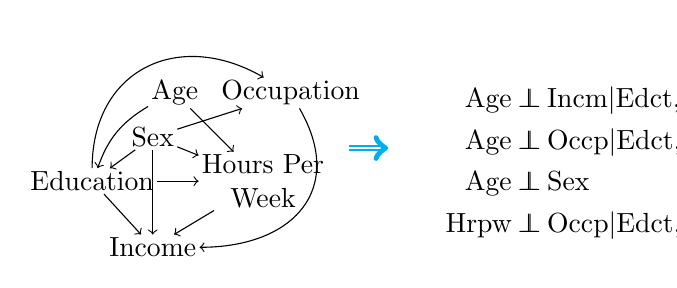
\begin{tikzpicture}
		\begin{scope}[xshift=-2.5cm, yshift=0.7cm, scale=0.7]
			\tikzstyle{every node}=[align=center, inner sep=1pt]
			\node (sex) at (-0.7, -0.8) {Sex};
			\node (age) at (-0.3, 0) {Age};
			\node (ed) at (-1.8, -1.6) {Education};
			\node (occ) at (1.8, 0) {Occupation};
			\node (hrpw) at (1.3, -1.6) {Hours Per \\ Week};
			\node (income) at (-0.7, -2.8) {Income};
		
			\draw[->]  (age) to[bend right=20] (ed);
			\draw[->]  (sex) to (ed);
			\draw[->]  (age) to (hrpw);
			\draw[->]  (ed) to (hrpw);
			\draw[->]  (sex) to (hrpw);
			\draw[->]  (ed) to (income);
			\draw[->]  (hrpw) to (income);
			\draw[->]  (occ) to[out=300, in=0, looseness=1.4] (income.east);
			\draw[->]  (sex) to (income);
			\draw[->]  (ed) to[out=90, in=150, looseness=1.3] (occ);
			\draw[->]  (sex) to (occ);	
		\end{scope}
		\begin{scope}[xshift=-3cm]
			\draw[thick, ->, double, cyan] (2.5,0) -- (3,0);
			\node[rectangle, align=center, inner sep=1pt] at (5, 0) {
				\begin{minipage}{.2\textwidth}
					\begin{equation*}
						\begin{split}
							\textnormal{Age} &\ci \textnormal{Incm} \rvert \textnormal{Edct, Hrpw, Sex} \\
							\textnormal{Age} &\ci \textnormal{Occp} \rvert \textnormal{Edct, Sex} \\
							\textnormal{Age} &\ci \textnormal{Sex} \\
							\textnormal{Hrpw} &\ci \textnormal{Occp} \rvert \textnormal{Edct, Sex} \\
						\end{split}
					\end{equation*}
				\end{minipage}
				};
		\end{scope}
		\end{tikzpicture}
		\caption{\todo[inline]{Finish figure. Show an example of model learnt using PC algorithm $\rightarrow$ Orienting the unoriented edges $\rightarrow$  Model testing}}
		\label{fig:ci_testing}
\end{figure}
\begin{figure}
	\caption{\todo[inline]{Take a model; show the modification indices for it.}}
\end{figure}

Inspired by this ranking approach in modification indices, in this paper we
develop a method to rank the CI tests using a conditional measure of
association. Our proposed approach uses the measure of association to find
correlated variables in the data that are not explained by the current model.
Using the measure, we can then rank the pair of variables between which adding
an edge would improve the explanation the most. Based on this information, the
user can select a potential pair of variables and based on their expert
knowledge decide the direction of the edge. 
\todo[inline]{Add about the score based methods somewhere here}

Our main contributions in this paper are as follows:
\begin{enumerate}
	\item We present a measure of (conditional) association for mixed data
		based on canonical correlations. This measure of association
		generalizes the widely used partial correlation to mixed data
		setting.
	\item Using this partial association measure, we present a procedure to
		rank CI tests. This ranking can be used to prioritize addition
		or deletion of edges from the model.
	\item Lastly, we present a web-browser based tool to allow researchers
		to apply this method to their own datasets.
\end{enumerate}

The rest of the paper is structured as follows. In
Section~\ref{sec:background}, we give a background on the measures of
association for various data types. In Section~\ref{sec:mixed_association}, we
present our method for computing mixed data association. In
Section~\ref{sec:modification} and Section~\ref{sec:web}, we present how to use
this method to make modifications and the web tool, and lastly in
Section~\ref{sec:empirical}, we show some empirical analysis on how well this
modification process works.

\section{Background and Related Work}
\label{sec:background}
We consider random variable $ X $ and $ Y $ with a possible multi-dimensional
variable $ \bm{Z} = \{ Z_1, \cdots, Z_k \} $. We consider these variables in
the mixed data setting where these variables can be any combination of
continuous, categorical, or ordinal unless specified. We also assume all
variables to be observed. We use $ \rvert \bm{Z} \rvert $ to represent the
cardinality of the variable $ \bm{Z} $. We write $ \bm{x} = (x_1, \cdots, x_n)
$ for a sample from $ X $ of size $ n $. We write the expectation of a variable
$ X $ as $ \mathbb{E}[X] $, conditional expectations as $ \mathbb{E}[X |
\bm{Z}] $.

We consider the problem of estimating the partial (or conditional) association
between $ X $ and $ Y $ in the presence of a set of conditioning variables $
\bm{Z} $. When $ Z = \emptyset $, this is equivalent to the marginal
association between $ X $ and $ Y $.

\subsection{Measures of (Conditional) Association}
\todo[inline]{Complete this section}
As our DAG construction procedure relies on a measure of conditional
association between variables, in this section we list out some of the already
known measures for specific data types. These measure of associations are
typically the effect size of various conditional indepdnence tests but they
don't need to be. However, there are no generalized measure of association for
mixed data, that we propose in the next section. This is by no means an
exhaustive list, rather just to give an idea of what can be done.

\paragraph{Both $ X $ and $ Y $ are continuous}
Where there are no conditional variables, $ \bm{Z} = \emptyset $, Pearson's
correlation coefficient can be used as a measure of association between the
variables. This does make various assumptions such as linearity between the
variables, normal distribution for $ X $ and $ Y $, and homoscedasticity.

In the case when $ \bm{Z} \neq \emptyset $, then partial correlations can be
used. This requires using two linear regression models: $ E_X: X \sim \bm{Z} $
and $ E_Y: Y \sim \bm{Z} $. Then computing the residuals using these two
regressions as: $ R_X = X - E_X(\bm{Z}) $ and $ R_Y = Y - E_Y(\bm{Y}) $. After
this a simple correlation coefficient can be computed between $ R_X $ and $ R_Y $.

\paragraph{All $ X $, $ Y $, and $ \bm{Z} $ are discrete}

In the case of discrete variables, Cramer\'s V has been typically used as a
measure of association. When there are no conditional variables, $ \bm{Z} = \emptyset $,
Cramer\'s V can be computed directly from the contingency table.

However, when conditional variables are present, we can iterate over all
possible combinations of the conditional variables, compute the Cramer\'s V and
then lastly combine them together. 

\paragraph{$ X $ is ordinal and $ Y $ is continuous}
Polyserial Correlation

When $ \bm{Z} = \emptyset $, ordinal variable can be assumed to be coming from
a thresholded normal distribution, estimate the thresholds and latent variable
to compute the correlation coefficient.

\paragraph{$ X $ and $ Y $ are ordinal}
Polychoric Correlation

\section{A Measure of Association for Mixed Data}
\label{sec:mixed_association}

In this section, we develop a novel partial measure of association for mixed
data by extending the idea of partial correlation to mixed data. As partial
correlations require two things: 1) A residualization method, and 2) measure of
associations between the residuals. We generalize this to mixed data by combining a
mixed data residualization method \citep{Ankan2023} with a multivariate measure
of association based on Pillai's Trace. Given $ n $ samples $ D = (x, y,
\bm{z}) $ of variables $ X $, $ Y $, and $ \bm{Z} $, we are interested in
computing an estimate of the conditional association $ \rho(X, Y; \bm{Z}) $
between $ X $ and $ Y $ conditioned on $ \bm{Z} $. As the residualization
approach requires atleast one conditional variable to be present, if $ \bm{Z} =
\emptyset $, we use a constant value for $ Z $. Similar to partial correlation,
we first compute the residuals for $ X $ and $ Y $ using $ \bm{Z} $ as the
predictor variables. We use the mixed data residualization approach from
\citet{Ankan2023}. Depending on the type of dependent variable, the residuals
are defined as follows:

\begin{enumerate}
	\item \textbf{Continuous:} We train a regression
		model, $ E_X: x \sim \bm{z} $. The residuals are then defined
		as the difference between the true and the predicted value using
		$ E_X $.
		$$ R_{x_i} = x_i - E_X(\bm{z}_i) $$
	\item \textbf{Ordinal:} We start by training a probability
		estimator, $ p_X: x \sim \bm{z} $, and take probability
		predictions from it $ \hat{p}_X: \hat{p}_X(\bm{Z}) $. Then we
		compute the residuals as follows:
		$$ R_{x_i} = \hat{p}(\hat{x}_i > x_i) - \hat{p}(\hat{x}_i < x_i) $$
	\item \textbf{Categorical:} We again start by training a
		probability estimator $ p_X: X \sim \bm{Z} $, and take the
		probability estimates from it $ \hat{p}_X: p_Z(\bm{Z}) $. Next,
		we one-hot encode the categorical variable and then compute the
		residuals as follows: 
		$$ R_X = x_i - \hat{p}(\bm{z}_i) $$
\end{enumerate}

\todo[inline]{Fix notations above}

Here, we have the option to choose the estimators based on the properties of
their data. Non-parametric ensemble estimators such as Random Forest and
XGBoost can work on any combination of data types while performing reasonably
well. For linear datasets we can also choose variants of linear regression
depending on the type of data. After the above steps are repeated for both $ X
$ and $ Y $, we end up with two residual matrices: $ R_X $ and $ R_Y $. The
type of the variable determines the shape for these matrices, i.e., if the
variable is continuous we get a residual matrix of shape $ ( n \times 1 ) $ and
if the variable is categorical we have a residual matrix of shape $ ( n \times
(k-1)) $ (where one of the dummy encoded variables is dropped to avoid
multicollinearity)

We now have two continuous valued residual matrices and the second step now is
to quantify the association between these residuals. In multivariate
statistics, canonical correlation based measures have been used for measuring
association between two sets of variables. We can treat the residuals as sets
of variables in case of categorical variable and use canonical correlations to
quantify the association between them.

\begin{definition}
	Given two sets of random variables $ \bm{U} = (U_1, U_2, \cdots, U_p) $
	and $ \bm{V} = (V_1, V_2, \cdots, V_q) $, canonical correlation between
	them, $\phi(\bm{U}, \bm{V}) $ is defined as:
		
	\begin{equation}
		\phi(\bm{U}, \bm{V}) = \sup_{a, b} \frac{a^T \Sigma_{\bm{U}\bm{V}} b}{\sqrt{a^T \Sigma_{\bm{U}\bm{U}} a} \sqrt{b^T \Sigma_{\bm{V}\bm{V}} b}}
	\end{equation}

\end{definition}
	
Canonical correlations are generalization of correlations to multi-dimensional
variables. It tries to find orthogonal linear transformations $ a $ and $ b $
of $ \bm{U} $ and $ \bm{V} $ such that the correlation between the transformed
variables $ a^T \bm{U} $ and $ b^T \bm{V} $ is maximized. It gives a vector of
correlation values of size $ \min(\rvert U \rvert, \rvert V \rvert) $
representing the correlation coefficient of each column of the transformed
variables. Pearson's correlation coefficient is a special case of canonical
correlations when $ \rvert U \rvert = \rvert V \rvert = 1$.

Many measures of association based on canonical correlation have been used in
multivariate statistics with each of them having slightly different properties.
\begin{itemize}
	\item Wilks' Lambda: $ \Lambda = \prod (1 - \phi_i^2) $
	\item Roy's Largest Root: $ \theta = \phi_{\max}^2 $
	\item Pillai's Trace: $ \tau = \sum \phi_i^2 $
\end{itemize}

We use Pillai's Trace for our purpose for two main reasons: 1) It uses all the
canoncial correlation values, 2) Its interpretation is similar to correlation
coefficient, i.e., $ 0 $ signifies no association and $ 1 $ signifies perfect
linear relationship. This gives us the following partial measure of association:

$$ \rho(X, Y; \bm{Z}) = \sum_{i=1}^{min(\rvert R_X \rvert, \rvert R_Y \rvert)} (\phi_i(R_X, R_Y))^2 $$


This measure of association has many desired properties:

\begin{enumerate}
	\item Bounded between $ 0 $ and $ 1 $.
	\item Independent of sample size.
	\item Invariant to the one-hot encoding scheme used fr categorical variables.
	\item Reduces to partial correlations when both variables are continuous.
	\item In case of discrete variables, connected to Cramer\'s V, a well
		known effect size measure for discrete variables.
\end{enumerate}
\todo[inline]{Expand on these points}

\section{Using Measure of Association for DAG Modification and Construction}
\label{sec:modification}

Using this mixed data partial association measure, we propose a method to rank
CI tests, and use it for model construction and modification. Given a
potentially empty DAG $ G $ and a dataset $ D $, for each pair for variable $ X
$ and $ Y $ in $ G $:
\begin{itemize}
	\item If there is no edge between $ X $ and $ Y $, we compute p-value for the CI test $ X \ci Y \rvert pa_G(X) \cup pa_G(Y) $ and the partial association measure: $ \rho(X, Y; pa_G(X) \cup pa_G(Y)) $.
	\item If there is an edge between $ X $ and $ Y $, we compute p-value for the CI test $ X \ci Y \rvert pa_{\underline{G}}(X) \cup pa_{\underline{G}}(Y) $ and the partial association measure: $ \rho(X, Y; pa_{\underline{G}}(X) \cup pa_{\underline{G}}(Y) $.
\end{itemize}

For a pair of variables $ X $ and $ Y $, if there is an edge present between
them, the interpretation of this partial association measure is similar to path
coefficients in SEMs, i.e. how strong is the edge between the variables. Hence,
we can use this to identify potential edges that can be removed from the model.
In the case when there is no edge between the variables, the value of this
partial measure of association can be interpreted as - given the current
structure of the model how much of the observed correlation between the
variables $ X $ and $ Y $ in data is not explained by the model. To modify the
model based on this, we can look at the pair of variables that have an edge
between them. If any of these pair have a p-value greater than partial
association below our chosen threshold, we can remove that edge as it is
redundant.

The measure of association also gives us a way to rank the potential
modifications. The smallest values (below the threshold) of the association
measure are the worst offending ones and for when the edges are not present the
largest values would add the most amount of explainability to the model. Using
this ranking the user can decide which pair of variables to focus on.

We can then use this to rank pair of variables which have very high unexplained
association between them. Based on the domain expertise, we can then choose one
of these suggested pair of variables, decide the direction of the edge between
the variables, and add it to the model. Once the new edge is added we can
recompute the association of all other variables and $ X $ and $ Y $.

Additionally, in each iteration of modification, for each pair of variable in $
G $, that has an edge between them in we compute the partial association
measure: $ \rho(X, Y; pa_{\underline{G}}(X) \cup pa_{\underline{G}}(Y) $. This
measure of association can be interpreted as the strength of the edge between
the variables. If the value of this association below a certain threshold, we
can remove the edge.

\todo[inline]{Add a figure showing an example of how this modification works.}

\begin{theorem}
	If we have access to an oracle that can give correct edge directions, taking a
	greedy approach with the procedure above results in the correct graph
	being recovered. \todo[inline]{Reword and add proof}
\end{theorem}

\section{Connection to score based methods}

\begin{itemize}
	\item Because they make only local changes, can get stuck in local minimas.
\end{itemize}

\section{Web Tool}
\label{sec:web}
Based on the procedure outlined in the previous section, we built a web-based
tool that allows us to interactively create/modify their model. The user
starts by uploading their dataset and optionally the initial DAG. If no initial
DAG is provided an empty graph is initialized. The tool also computes the
Shipley's C value at any point. The web-tool would automatically show all
unexplained associations in the DAG by adding red edges between them. The edge
weight of the edge represents how high this strength is. Users can also set the
threshold for p-value and association to control how many edges are shown at a
time. Based on these shown potential edges, the user can select the edge that
they want to add and decide the direction for it. If the tool detects an
incorrect edge in the graph, it is shown in black. Once the user is happy with
the graph they have they can export it into different formats to use it for
further computation.

\todo[inline]{Add screenshots here}

% \begin{figure}
% 	\centering
% 	\begin{subfigure}{0.5\textwidth}
% 		\includegraphics[scale=0.25]{../../presentations/2024_05_das/2.png}
% 	\end{subfigure}%
% 	\begin{subfigure}{0.5\textwidth}
% 		\includegraphics[scale=0.25]{../../presentations/2024_05_das/5.png}
% 	\end{subfigure}
% 	\caption{Screenshots of the web-tool. \todo[inline]{Insert screenshots of the web-tool}}
% \end{figure}

\section{Empirical Analysis}
\label{sec:empirical}

\begin{figure}
	\begin{subfigure}{0.5\textwidth}
		\centering
		\includegraphics{../code/plots/shd_ribbon.pdf}
		\caption{}
	\end{subfigure}
	\begin{subfigure}{0.5\textwidth}
		\centering
		\includegraphics{../code/plots/sid_ribbon.pdf}
		\caption{}
	\end{subfigure}
	\caption{Comparison of PC and Hill-Climb Search algorithms against
		manually drawn DAGs using the assistance method. As PC and
		Hill-Climb Search return the Markov Equivalence Class (MEC), we
		use the best and worst scoring orientation of the MEC to get
		the range of values. The human drawn values are done for
	multiple accuracy values of the oracle. \todo[inline]{Replace Hill-Climb with GES and improve the plot}}
\end{figure}

We analyzed the performance of this manual approach by comparing it with two
automated algorithms: PC and Greedy Equivalence Search (GES). For the
comparison we use simulated data from a known DAG and compare how well the
algorithm is able to recover the original model using two metrics: Structural
Hamming Distance (SHD) and Structural Intervention Distance (SID). To simulate
the data, we start with a randomly generated DAG on $ 10 $ nodes and use linear
models with random effects to generate the data. 

We vary the edge probability of the DAG to generate DAGs with varying density.
We repeat the data generation $ 30 $ times for each density value for the DAG.
As both PC and Hill-Climb Search can only give us a CPDAG, we compare the
orientation of these CPDAG which result in the best and worst case scores on
SHD and SID.

To use our proposed approach, we need an expert to tell us the direction of the
edges. We simulated an expert using this assisted model construction approach,
we start with an empty model and take a greedy approach to add edges to this
model. At any point, we select the pair of variables that has significant
correlation and the highest unexplained correlation, i.e., highest conditional
association. We then use an oracle to decide the direction of the edge between
the variables. Given an accuracy of the oracle, $ \alpha $, the oracle either
gives the correct direction, incorrect direction, or returns None representing
that it does not know the direction.

\begin{equation}
	\begin{split}
		x &= \textnormal{rand}([0, 1]) \\
		O(\alpha) &= \begin{cases} 
			M \rightarrow Y, & \textnormal{if  } x <= \alpha \\
			\textnormal{rand}(M \rightarrow Y, M \leftarrow Y, None) & \textnormal{otherwise} \\
				\end{cases} \\
	\end{split}
\end{equation}

If the oracle returns None for any pair of variables, an edge between this pair
is not suggested to the oracle in future iterations. We also make sure that
only edges which do not form a cyclic in the graph are used to select the next
potential edge. After adding each edge, we also check if the p-value of any
existing edge shows independence. If that happens we remove that edge and
blacklist that edge, i.e., that edge is not prompted again during the run of
the algorithm. We repeat this procedure till the model explains all
correlations between the variables. There is a possibility that this greedy
expert gets stuck at incorrect graph structures as it does not do any
backtracking to fix its earlier mistakes. This procedure is outlined in the
Algorithm 1.
\todo[inline]{Show an algorithm of how this expert method is working}

\subsection{Using Large Language Models as Experts}
A lot of recent work has focused on finding pairwise causal direction among
variables using Large Language Models. In this analysis, instead of using the
oracle to decide the direction of edges, we used GPT4 to give us the direction
of the edges based on description of the variables. As GPT4 has already
memorized many of these models, we encoded the variable names using a random
string and provided the description of the variable to let it decide the
direction of the edge.

\begin{figure}
	\centering
	\begin{subfigure}{0.5\textwidth}
		\caption{\todo[inline]{Add the prompt used}}
	\end{subfigure}
	\begin{subfigure}{0.5\textwidth}
		\centering
		\includegraphics[scale=0.3]{../code/plots/llm_adult.png}
		\caption{\todo[inline]{Change figure to have consistent style}}
	\end{subfigure}
\end{figure}

\section{Conclusions}

\newpage
\bibliography{references}
\end{document}
